\chapterimage{Detector/DetFigures/VirgoTube.jpg} % Chapter heading image
%Einstein Telescope artits impression copyright Nikhef
\chapter{Detector}
\label{chap:Detector}

%**********************************************
\section {Optical Layout}
% Authors R.Flaminio, A. Freise, S.Hild
\label{Sec:Layout}
\FloatBarrier
\label{sec:optlayout}

\begin{wrapfigure}{r}{0.4\textwidth}
%\begin{figure}{H}
	\centering
	\includegraphics[width=0.3\textwidth]{Intro/Intro_Figures/NestedDetectors.pdf}
	\caption{Three nested detectors in a triangular arrangement will 
	form the final Einstein Telescope geometry.}
	\label{fig:NestedDetectors}
\end{wrapfigure}
In its final construction stage the Einstein Telescope will consist of three
nested detectors, which will be arranged in a triangular pattern as shown in
figure\,~\ref{fig:NestedDetectors}. In contrast to the traditional L-shaped
geometry of the first and second generations of gravitational wave detectors
this arrangement is equally sensitive for both polarisations of the
gravitational wave. Additionally it shows a more isotropic antenna pattern
compared to the L-shaped detectors.%, as shown in figure\,~\ref{fig:response}. 
The
overall frequency range covered will reach from a few Hertz to about 10\,kHz.

Each individual detector in turn will comprise two interferometers, one
specialised for detecting low-frequency gravitational waves and the other one
for the high-frequency part of the spectrum. The sensitivity goal for each interferometer is
shown in figure\,\ref{fig:ET_sensitivity}. %\\ 
Each individual interferometer has a  dual-recycled Michelson topology with
Fabry-Perot arm cavities. This is a mature and well tested configuration
currently employed  second-generation detectors, such as Advanced LIGO and
Advanced Virgo. 

This section describes the details of the ET optical layout, such as the laser
beam sizes, beam shapes and distances between optical components inside the arm
cavities and central interferometer including the power and signal recycling
cavities. A schematic sketch of the optical layout of all core optical of the
interferometers is shown in figure~\ref{Fig:Simple_ETv1}. 

\begin{figure}[p]
\centering
\includegraphics[width=0.9\textwidth]{Detector/Optics/OpticalLayout/OpticalLayoutFigures/ET_April2011_v2.png}
\caption{\tcb{PICTURE TO BE REPLACED BY UPDATED LAYOUT. Will probably choose something with more details on the infrastructure  (tunnels, shafts etc) and less details on what is inside vacuum system} Simplified drawing of the low and high frequency core interferometers of a single ET-detector. Injection and detection optics as well as filter cavities have been omitted for clarity. Please note that the complete ET observatory consists of three such detectors.%
}
\label{Fig:Simple_ETv1}
\end{figure}

\subsubsection{A xylophone design for ET}\label{sec:xylophone} 
Spanning the detection band over four orders of magnitude in frequency, as is
asked for third-generation GW observatories such as ET, is technically extremely
challenging: different noise types dominate the various frequency bands and
often show opposite responses for different tuning of the same design parameter.

In the following we provide examples of fundamental issues of a broadband
third-generation interferometer that could be resolved by using a set of
xylophone detectors~\cite{Hild2010a}:
\begin{itemize}
\item \textbf{Control Noises}: Many noise sources limiting the second generation
GW detectors at the low frequency end seem to become more challenging with
increased optical power: classical radiation pressure forces and torques
originating from residual misalignments and beam jitter dominate the dynamics of
the interferometer mirrors and hence the local and global control loops. 
The xylophone concept will help ET to achieve its unprecedented low-frequency
sensitivity target, by minimising the radiation pressure driven forces on the
mirrors of the ET LF detector. 
%Similarly, thermal deformation of the main
%optics at high optical power are currently a challenge for achieving low 
%optical losses during operation. 
\item \textbf{Shot Noise vs Radiation Pressure Noise}: Due to the fact that the
shot noise contribution scales inverse with optical power, but the photon
radiation pressure noise contribution on the other hand scales proportional to
the optical power, it will be hard to obtain the desired bandwidth with a
single detector. Therefore, again it might be useful to split ET into a
low-power low-frequency and a high-power high-frequency companion.
\item \textbf{High Power vs Cryogenic Temperature}: In a single broadband ET
observatory the simultaneous use of high optical power (a few megawatts) to
achieve the required high frequency sensitivity and test masses at cryogenic
temperatures in the 10 to 20\,K range in order to provide the required
suppression of thermal noise would pose a strong challenge. Even though tiny,
the residual absorption of the dielectric mirror coatings deposits heat in the
mirrors which is difficult to extract, without spoiling the performance of the
seismic isolation systems. A possible solution for this problem would be to
build a xylophone observatory consisting of a high-frequency detector featuring
high power and high temperature, and a low-frequency detector featuring low power
and cryogenic temperatures.
\end{itemize}

The xylophone concept was first suggested for Advanced LIGO, proposing to
complement the standard broadband interferometers with an interferometer
optimized for lower frequency, thus enhancing the detection of high-mass binary
systems \cite{Shoemaker2001LIGOXylophone, Conforto2004}.
One may think that a xylophone might significantly increase the required
hardware and its cost by the need to build more than one broadband instrument.
However, such an argument does not take the technical simplifications that it
would allow, the better reliability of simpler instruments, and the more
extensive scientific reach allowable into account.

\begin{comment}
For example splitting a third-generation observatory into a low-power,
low-frequency  and a high-power high-frequency interferometer, has not only the
potential to resolve the above mentioned conflict of photon shot noise  and
photon radiation pressure noise, but also allows to avoid the combination of
high optical power and cryogenic test masses. To reduce thermal noise to an
acceptable level in the low frequency band, it is expected that cryogenic
suspensions and test masses are required. Even though tiny, the residual
absorption of the dielectric mirror coatings deposits a significant amount of
heat in the mirrors. Since this heat is difficult to extract, without spoiling
the performance of the seismic isolation systems, it imposes a limit on the
maximum circulating power of a cryogenic interferometer.
\end{comment}

\begin{figure}[thbp]
\centering
\includegraphics[width=0.8\textwidth]{Detector/Optics/OpticalLayout/OpticalLayoutFigures/Layout_overview.pdf}
\caption{Simplified sketch of the ET low and high frequency core interferometers of a single ET-detector.}
\label{Fig:opt_lay_over}
\end{figure}

\begin{table}
\begin{center}
\begin{tabular}{l l l}
\hline
\hline
Parameter & ET-D-HF   & ET-D-LF \\
\hline
Arm length & 10\,km & 10\,km \\
Input power (after IMC) & 500\,W & 3\,W \\
Arm power & 3\,MW & 18\,kW\\
Temperature & 290\,K &  10\,K  \\
Mirror material & fused silica & silicon \\
Mirror diameter / thickness & 62\,cm / 30\,cm & min 45\,cm/ \tcb{(TBD)} \\
Mirror masses & 200\,kg & 211\,kg \\
Laser wavelength & 1064\,nm & 1550\,nm \\
SR-phase & tuned (0.0) & detuned (0.6)\\
SR transmittance & 10\,\% & 20\,\% \\
Quantum noise suppression &  freq.\ dep.\ squeez.& freq.\ dep.\ squeez.\\
Filter cavities & $1 \times $300\,m  & $2 \times$ 1.0\,km \\
Squeezing level  & 10\,dB (effective) & 10\,dB (effective) \\
Beam shape & TEM$_{00}$ & TEM$_{00}$\\
Beam radius & 12.0\,cm & 9\,cm \\
Scatter loss per surface & 37.5\,ppm & 37.5\,ppm \\
Seismic isolation & SA, 8\,m tall & mod SA, 17\,m tall \\
Seismic (for $f>1$\,Hz) & $5\cdot 10^{-10}\,{\rm m}/f^2$ & $5\cdot 10^{-10}\,{\rm m}/f^2$  \\
Gravity gradient subtraction & none \tcb{(TBC)} & none \tcb{(TBC)}\\
\hline
\hline
\end{tabular}
\caption{Summary of the most important parameters of the ET-D high and low frequency interferometers. SA~=~super attenuator,  freq.\ dep.\ squeez.~=~squeezing with frequency dependent angle. \label{tab:summary14}}
\end{center}
\end{table}

The baseline for ET is a 2-band xylophone detector configuration, composed of a
low-frequency (ET-LF) and a high-frequency (ET-HF) detector. Both
interferometers are Michelson interferometers featuring 10\,km armlength and an
opening angle of 60 degrees.  Due to their similar geometry both detectors will
share a single facility. Table~\ref{tab:summary14} gives a brief overview of the
main parameters of the analysed low-frequency (ET-LF) and high-frequency (ET-HF)
detector. Figure~\ref{Fig:opt_lay_over}   shows sketches of the corresponding
core interferometers and the filter cavities. The full layout of the two core
interferometers of a single ET detector is depicted in
Figure~\ref{Fig:Simple_ETv1}.

% -------------------------------------------------------------------------------------------
\subsubsection{Arm cavity design}
\label{sec:arm_cavity_design}
The size and shape of the laser beam inside the interferometer is defined by the
surface shape of the cavity mirrors; the beam sizes at the arm cavity input
mirrors (IM) and arm cavity end mirrors (EM) as well as the position of the
cavity waist are determined by only two parameters, the radii of curvature (ROC)
of IM and EM. Since inside the two Fabry-Perot cavities of the Michelson
interferometer the GW interacts with the laser light, creating signal sidebands,
the two arm cavities can be seen as the heart of the ET interferometers. The
characteristics of the arm cavities have not only a high impact on the detector
sensitivity and bandwidth, but also on the overall detector performance.


The choice of the beam size on the arm cavity mirrors is a trade-off process
taking the following considerations into account:
\begin{itemize}
%  \item For a given cavity length there is a minimal achievable beam size, which
%  is determined by the divergence of the beam.
\item Above a minimal beam size, given by the length of the interferometer arm,
any further increase in beam size leads to a reduction of the various 
thermal noise contributions from the cavity mirrors.
\item The upper limit for the manageable beam size is given firstly by
the maximum available mirror substrate size and secondly by the approaching of
the cavity instability.
\end{itemize}

%\textbf{Arm cavity mirror size}
A common method to define the mirror size is to demand the optical power loss
due to clipping (light being lost because it `falls over the edge of the
mirror') to be less than $1\,$ppm. This results in a scaling factor between 
beam and mirror radius of 2.63 (for TEM$_{00}$ modes), see~\cite{Chelkowski2009}.

\begin{comment}
\begin{center}
\begin{tabular}{|l|c|c|}
	\hline
	mode  & TEM$_{00}$ & LG$_{33}$\\
	\hline
	mirror radius to beam  radius & 2.63 & 4.31\\
	\hline
\end{tabular}
\end{center}

\textbf{Minimal mirror sizes for ET}

Using the currently discussed options for ET we can compute minimal mirror sizes
for various options, by using $L=R_{C}$ resulting in $w_{\rm
min}=\sqrt{\frac{L\lambda}{\pi}}$.
\begin{center}
\begin{tabular}{|l|c|c|}
	\hline
setup & min beam radius  & min mirror diameter \\
         & [cm] & [cm] \\
	\hline
LG$_{33}$, 1064\,nm  &  5.8      &  50.2     \\
	\hline
TEM$_{00}$, 1550\,nm  &  7.0      &   37.0    \\
	\hline
\end{tabular}
\end{center}

\textbf{Realistic mirror sizes for ET}

The minimal beam size can be computed using $L=R_{C}$ resulting in 
$w_{\rm min}=\sqrt{\frac{L\lambda}{\pi}}$ as:
\begin{center}
\begin{tabular}{|l|c|c|}
	\hline
wavelength & min beam radius  & min mirror diameter \\
         & [cm] & [cm] \\
	\hline
1064\,nm  &  5.8      &  30.6     \\
	\hline
1550\,nm  &  7.0      &   37.0    \\
	\hline
\end{tabular}
\end{center}

\textbf{Realistic mirror sizes for ET}
\end{comment}

Using the minimal beam sizes is obviously not optimal in terms of thermal noise.
Therefore we intend to push the beam sizes for ET towards the maximum feasible
size, which corresponds to about 60\,cm substrate diameter for fused silica
mirrors and 45\,cm for the silicon mirrors. Assuming 10\,km long arm cavities,
we can derive the following arm cavity characteristics.

\begin{center}
\begin{tabular}{|c|c|c|c|c|c|c|c|c|}
  \hline
IFO & $\lambda$& beam & mirror $\varnothing$ & $R_{\rm C}$ & $w_0$ &$z_0$ & $w$ & $g-$factor \\
\hline
ET-HF & 1064\,nm & TEM$_{00}$ & 62\,cm & 5070\,m & 1.42\,cm & 5000\,m & 12.0\,cm & 0.95\\
\hline
ET-LF & 1550\,nm & TEM$_{00}$ & 45\,cm &5580\,m & 2.9\,cm & 5000\,m & 9.0\,cm & 0.63\\
\hline
\end{tabular}
\end{center}

% ----------------------------------------------------------------------------------------------------

\FloatBarrier
\subsubsection{Central interferometer design}
\label{sec:opt_layout_CITF}

The central interferometer consists of the two recycling cavities and the
central Michelson interferometer formed by the beam splitter and the arm cavity
input mirrors. The design of the central interferometer is mainly determined by
two constraints. First of all it should allow for the implementation of
non-degenerate recycling cavities. Second, the central interferometer has to
serve as mode-matching telescope for the arm cavities.

The non-degenerate recycling cavity design used by the advanced detectors 
%(see Figure~\ref{Fig:Sec_Optics_AdvLIGO_IFO_Schematic}) 
can probably not be directly
adapted for ET, because no beam splitter substrates of the required dimensions
would be available. For example the high frequency interferometer featuring an
opening angle of 60 degree would require a beam splitter with a diameter of
more than 120\,cm.

Therefore we plan to investigate design options making use of input mirror
substrates including a focussing lens and introducing a two telescope 
mirrors in a z-configuration between the IMs and the central beam
splitter, see~\ref{Fig:mode_matching_telescope}.
Please note that the arm cavity mirrors are \tcb{(comment nchriste:) and?'} possibly the telescope mirrors are
the only full sized optical elements and that the beam splitter and recycling
mirrors  can be significantly smaller.

\begin{figure}[thbp]
\centering
\includegraphics[width=0.4\textwidth]{Detector/Optics/OpticalLayout/OpticalLayoutFigures/telescope_drawing.pdf}
\caption{Simplified sketch of mode matching telescopes in the interferometer
arms.
\bluecomment{Replace this image with a cleaner sketch.}}
\label{Fig:mode_matching_telescope}
\end{figure}

\begin{comment}
\textbf{Layout option for TEM$_{00}$, 1550\,nm}
\nopagebreak

The optical parameters of a possible solution based on a arm cavity length of
$L=10$\,km and a TEM$_{00}$ mode at 1550\,nm are provided below:
\begin{itemize}
\item focussing element in or near the ITM with a focal length of $f=303$\,m
\item distance ITM--BS: 300\,m
\item distance BS--MPR: 10\,m
\item beam size on BS: 6\,mm
\item beam size on MPR: 3.4\,mm
%\item Rayleigh range in central interferometer: 6.3\,m
\end{itemize}

The recycling cavity formed by MPR and ITM has a length of 310\,m and a free
spectral range of 484\,kHz. The round-trip Gouy phase is given by $\approx
9.6$\,deg which corresponds to a mode separation frequency of $25.8$\,kHz.

\textbf{Layout option for LG$_{33}$, 1064\,nm}
\nopagebreak

Using the same distances and focussing elements for the interferometer with a
LG$_{33}$, 1064\,nm beam, we also obtain reasonable numbers:
\begin{itemize}
\item beam size on BS: 4.7\,mm
\item beam size on MPR: 2.7\,mm
%\item Rayleigh range in central interferometer: 6.7\,m
\item Gouy phase: 10.5\,deg
\item mode separation frequency:  28.1\,kHz
\end{itemize}

These layout options are not yet optimised but they show that a separation
between beam splitter and input optics in the order of 300\,m represents a
useful baseline. The numbers for the beam sizes at the beam splitter and
recycling mirrors in both cases need to be checked against a detailed thermal
noise computation.

Furthermore, the design needs to be evaluated for losses originating from
astigmatisms inside the recycling cavities as well as for scattered noise
issues.
\end{comment}






\section{Optics and Interferometry}
% Authors R.Flaminio, A. Freise, S.Hild
\label{Sec:Optics}

\subsection{Core Optics and Coatings}
\label{Sec:CoreOptics}
This section focuses on the mirrors forming the arm cavities of the interferometer (IM and EM). Those optics, also called test masses, are the largest and most critical ones whose displacement noise can directly degrade the gravitational waves signals.

To ensure the best optics, the three ingredients of a mirror: substrate, polishing and coating will have to use state of the art technologies. An overview of current achievements and the core optics strategy for ET is presented in the following sections. The working temperature of the optics have a strong impact on the technological choices to be made. 

\subsubsection{The substrate materials}

The substrate of the large optics must meet some drastic specifications in term of optical and mechanical specifications, moreover it should be available in large sizes and it must be shaped to the atomic level. Due to such constraints, few specific materials can be considered: fused silica for room temperature interferometer and sapphire and silicon for cryogenic temperature.\\

\paragraph{Fused silica} is the substrate of choice for all the current room temperature interferometers.  Due to its extensive
use for first and second generation gravitational wave detectors, this material has been extensively characterised at room temperature. Moreover the polishing and coating are now well mastered for this material \cite{pinard2017mirrors}.

Fused silica is transparent in the visible and near infrared, the operating wavelength of room temperature ET will be 1064~nm, the same as advanced interferometers. At this wavelength fused silica exhibits very low bulk optical absorption (below 1 ppm/cm) with high homogeneity of refractive index (relative optical path length < 0.1 nm/cm over the central part) and very low birefringence (around 1 nm / cm). The material can be isotropic in 3 dimensions which is ideal for the central beansplitter where laser beams are crossing the substrate at different angles.

In addition to its outstanding optical properties, fused silica presents a very low Brownian thermal noise at room temperature. Additionally, there exist techniques to fabricate quasi-monolithic suspensions based on pulled fused silica fibres and silicate bonding to further reduce the suspension thermal noise. These techniques have demonstrated their reliability and performances for years in the GEO600 detector \cite{plissi1998aspects} and so have been successfully implemented in LIGO and Virgo detectors \cite{robertson2002quadruple,lorenzini2010monolithic}.

The upgrade of Advanced Virgo, called Advanced Virgo+ will use test masses in fused silica of diameter 55~cm weighting 100~kg, that would be similar to the optics for ET-HF which will be in the same material and with a diameter of 62~cm for 200~kg. Hence, fused silica as a large optical substrate presents the best performances at room temperature with a very limited risk.\\


\paragraph{Sapphire} is considered as a substrate candidate for ET-LF since as a monocrystal it is well suited for low temperature optics. Sapphire crystals have exceptional physical properties, impressive hardness (only exceeded by diamond), large optical transmission from visible to infrared and large resistances to thermal shocks and chemicals.

One crucial point about operating at low temperature is the constraint on the substrate optical absorption. The heat generated by the passing laser beam increases the test mass temperature and it can only be efficiently removed through the thin suspension fibers. Measuring the optical absorption at 1064~nm of several large  sapphire ingots has shown the disparity of the results, very low optical absorption ($<$ 50 ppm/cm) can never been granted and could only be achieved after selection of the best substrates. The current best sapphires were used as KAGRA input mirrors of the arm cavities, with a diameter of 22 cm for a thickness of 15~cm, they present an absorption of around 40~ppm/cm \cite{PhysRevD.89.062003}.  

To strongly reduce the birefringence, special care must be taken to ensure that the optical axis is well aligned with the c-axis of the crystal. Substrate refractive index inhomogeneity is larger than in fused silica but it can be compensated during the polishing process for transmissive optics. 

Low thermal noise can be expected from sapphire substrates at low temperature. The thermo-elastic noise is strongly reduced thanks to the decrease of the thermal expansion coefficient ($\alpha = 1 \times 10^{-9}$ [K$^{-1}$]\cite{taylor1996measurement} at 10~K) and a bulk mechanical loss of $ 5 \times 10^{-9}$ (10~K) was measured ensuring a low substrate Brownian thermal noise \cite{uchiyama1999mechanical}.

Sapphire is currently used in KAGRA the Japanese cryogenic interferometer and the experience acquired by operating such optics at low temperature is full of insights \cite{Akutsu_2019}. In particular, the issue of a growing thin layer of ice on the optics which increases the optical losses in the arm cavities was highlighted \cite{hasegawa2019snow} and the impact on thermal noise later estimated \cite{PhysRevResearch.1.013008}. This issue could be mitigated by lowering the pressure in the long arm vacuum pipes and increasing the cold vacuum duct (working as a cryotrap) in front of the mirrors. The necessity for the substrate of the mirrors to be precisely along the c-axis was also demonstrated as it could lead to detrimental birefringence and imperfect correction of the refractive index inhomogeneity, both synonymous of optical losses \cite{somiya2019birefringence}. 

The largest incertitude regarding sapphire substrate for ET-LF is the availability of 200~kg ingot with extremely good optical properties, in particular too high optical absorption (few tens of ppm/cm) could be a showstopper. Sapphire boules above 200~kg are currently produced (to be cut in wafer for LED substrates) \cite{Bigspapphire2019} but the overall optical quality and uniformity are still to be demonstrated considering the ET requirement.\\

\paragraph{Silicon} is the second candidate material for the test masses for the cryogenic interferometer ET-LF. Compared to fused silica and sapphire materials presented previously, silicon is not transparent at 1064~nm and so the operating wavelength of the detector has to be shifted to 1550~nm. 

Silicon has excellent mechanical and thermal properties and is easily available in relatively high quality due to the large market of the semiconductor industry. The coefficient of thermal expansion is zero at two special temperatures around 18~K and 125~K \cite{lyon1977siliconexpansion}. At these temperatures the contribution of thermo-elastic noise will therefore vanish. The mechanical loss of silicon has been studied by Q-factor measurements. It was experimentally shown that silicon bulk samples can reach mechanical losses as low as $1 \times 10^{-9}$ at 10~K. \cite{mcguigan1978siliconQ}.

The maximum available diameter and purity of silicon depends on the fabrication process. The two main growing processes for single crystal silicon used by the semiconductor industry are the Czochralski (CZ) and the Float Zone (FZ) methods. CZ silicon is grown from a silicon melt in a silica crucible. It results in
relative large samples with a reasonable purity. The most dominant impurities in undoped CZ-grown silicon are carbon (typically 10$^{-18}$ cm$^{-3}$) and oxygen (typically up to 10$^{-19}$ cm$^{-3}$). 

In contrast, FZ silicon contains also these impurities but in much smaller concentrations (up to 10$^{-3}$ times smaller). During the FZ growth process, single or poly-crystalline silicon is remelt by means of inductive heating in vacuum or under an inert atmosphere. Impurities dissolve better in the melt than in the solid part. The re-crystallised material has therefore a higher purity than the initial one. By slowly sweeping the melt from one end to the other it is possible to purify in steps. The mechanism of inductive heating sets limits to the currently available setups and leads to smaller currently available samples.

Using the CZ growth technique, silicon ingots up to 45~cm of diameter can be produced however 30~cm is still the dominant wafer diameter in the semiconductor industry. For FZ silicon the diameter is currently limited to 20~cm.

In the recent years, motivated by the possible use of silicon as test mass materials, the optical properties of silicon have been thoughtfully characterised. Regarding the bulk optical absorption at 1550~nm, it was demonstrated the direct link between impurities concentration and the absorption \cite{degallaix2013abs_silicon}. For FZ silicon, absorption below 5~ppm/cm has been measured which is compatible with the ET-LF requirement. During the absorption studies, excess optical absorption at the surface of silicon was reported \cite{khalaidovski2013indication} which is likely linked to the polishing techniques used and not intrinsic to the material \cite{bell2017Sisurf}. According to the latest measurement, magnetic Czochralski (mCz) growth technique would be the most suitable approach for ET as it can combine large diameter ingot (45~cm diameter) with very low impurities since absorption around 20~ppm/cm has been achieved on one sample.

Thanks to the very low intensity of the laser beam in ET-LF, non linear effects such as two photon absorption \cite{bristow2007two} or Kerr effect are expected to be negligible.

Other caracterisations done in the framework of the Einstein Telescope include the measurement of thermo-optic coefficient at low temperature \cite{komma2012SithermoOptic} which is essential to derive the thermal lensing magnitude and the substrate thermo-refractive noise and also the birefringence \cite{kruger2015birefringenceSi} which is in the same order of magnitude as for sapphire. 

Like for sapphire, the choice of silicon substrate for ET-LF will be validated when it could be demonstrated that this material can come in large size (diameter of 450~mm) together with a very low optical absorption (order of several ppm/cm) at 1550~nm. Silicon ingot made with mCz seems to meet those specifications on some sample but the repeatability has yet to be proven.

\subsubsection{Surface polishing achievement}

The polishing capability will depend on the substrate material. Polishing of fused silica is well mastered thanks to current generation of room temperature interferometers and hence presents little risks. For the Einstein Telescope, the same flatness and roughness that was achieved \footnote{flatness inferior to 0.5~nm RMS and roughness below 0.1~nm RMS on the central part \cite{pinard2017mirrors}.} for Advanced detectors should be enough albeit on a larger area since the ET mirrors will be bigger. Due to the heavier substrate, special handling tools will have to be manufactured but according to the polishing companies, there is no showstopper. The large end mirrors of Advanced Virgo+ with a diameter of 550~mm and weighting 100~kg will be a pertinent pathfinder before the procurement of the ET mirrors.

Sapphire which is one the hardest known material has always been very difficult to polish. Until recently, pushed by the mirror requirement from KAGRA, a surface quality as good as the one for fused silica has been demonstrated \cite{hirose2014sapphire}. This a tremendous achievement even at the price of a larger cost and longer delay compared to fused silica.


independent of temperature! what we have achieved right now, size, surface quality
Should not be an issue.
Silicon more brittle.

\subsubsection{The coating materials and design}

A quick reminder of the problem (the longer version is in the original study). Focus on the coating thermal noise
Formula, thermal noise depends on temperature, beam size, coating loss angle

focus on the latest progress (multi-materials approach, promising materials),
Planned strategy to achieve what we want for ET

Already Ok for room temperature ?

\subsubsection{Thermal noise curves}

noise curve in this section similar to figure 187 from original study, tell explicitly which parameters have been updated to derive the curves

\paragraph{LF interferometer}

\paragraph{HF interferometer}


\subsubsection{Other core optics}

Central interferometer optics such as Power and Signal Recycling Mirrors (PRM and SRM) or Beamsplitter will be smaller in size (diameter in the order of 10~cm) and at room temperature. Fused silica is hence the preferred material for the substrates. The coating will use the same materials as for ET-HF to benefit from state of the art deposition process. The procurement of those optics does not represent any challenges and will be straightforward.

%\subsection{Coatings}
%\input{Detector/Optics/Coatings/Coatings.tex}

\subsection{Light sources}
\label{Sec:Lasers}
% Author H.Lueck

\subsection{Quantum noise reduction}
\tcb{ET design, 5.5, also D3 (filter cavity)}
% interferometer configuration, squeezing, 
\label{Sec:Squeezers}
% Author H.Lueck

%\subsection{Auxilliary Optics}
%\input{Detector/Optics/AuxOptics/AuxOptics.tex}

\subsection{Interferometer control}
\tcb{does not exist yet}



To operate GW interferometers such as ET, many degrees of freedom (DOFs) need to be controlled. 
The most important DOFs belong to the interferometer as a whole, and can be divided into the longitudinal DOFs, which involve controlling the position of the main mirrors along the optical axis, and the angular DOFs which refer to the orientation of the main mirrors with respect to the incident beam axis. 
There are several more control loops, the auxiliary loops, which control e.g. the position or velocity of some part of a suspension, or the power of the laser system, but we mostly focus on longitudinal and alignment control here, since these are most critical for the overall performance of the interferometer.

Regardless of the split in longitudinal and alignment control,
some links between them exist too, such as the bi-linear coupling of alignment control noise with
beam spot position on test masses into the longitudinal signals. We will point these out where required.


\subsubsection{Longitudinal control}

In the steady-state operation of the interferometer, longitudinal control is concerned with maintaing longitudinal DOF's relevant to keep the interferometer and optical cavities at (or sufficiently close to) their nominal operating points. Another distinctive task of longitudinal control is lock acquisition, which is the process of bringing the interferometer reliably to its steady-state operating point.

For a single Fabry-Perot cavity, consisting of two or more mirrors, the standard way to obtain an error signal for locking the cavity to resonance with the incoming laser light, is the Pound-Drever-Hall technique \cite{Drever1983}. The technique consists of adding RF sidebands to the optical frequency of the laser using a modulator. Alternatively modulation can also be applied to the cavity itself, e.g. by modulating the round-trip length of the cavity. The signal in reflection of the cavity is then demodulated yielding a signal proportional to the deviation from resonance. This error signal can be used to control the length of the cavity by e.g. actuating on the mirror, or to control the laser frequency. This is a system with a single DOF and is applied for input mode-cleaners and output mode-cleaners of current GW interferometers, with sufficient performance to also be suitable for ET.

A GW interferometer is more complex than a single cavity, and has more longitudinal degrees of freedom. 
The number of DOF's for the main interferometer is determined by the number of optical resonators that form
the interferometer (plus one for controlling the interference condition of the Michelson interferometer). Typically there are more suspended mirrors than DOFs which leaves some of them uncontrolled, as for example a global translation of all mirrors or the relative position of folding mirrors within recycling cavities (the latter may be controlled for ET if required, to reduce scattered light from moving fringe patterns on folding mirrors).

The first generation ITFs (called PRFPMI), such as initial LIGO and Virgo consisted of 4 DOFs: Differential Arm length (DARM), consisting of the length difference of the two long arm cavities, Common mode ARM length (CARM), the length sum of the two long arms, the Michelson DOF (MICH) and the Power Recycling Cavity Length (PRCL). For the second generation detectors advanced LIGO, advanced Virgo and KAGRA, a fifth DOF is added: Signal Recycling Cavity Length (SRCL), which will also be the case for the ET interferometers.

%[xx figure with DOF definition, ports]

Of these five DOFs, the DARM loop is of particular importance, since it directly contains the information of gravitational wave signals. This means that greatest care is taken to bring the noise performance of the corresponding readout to the most fundamental limits of the given configuration.
Since this DOF is also actively controlled, the effect of the corresponding feedback loop must be taken into account to obtain a calibrated gravitational-wave signal that can be used for data analysis.

The operation of the Advanced LIGO and Advanced Virgo interferometers
has demonstrated the feasibility of longitudinal control techniques for second generation detectors.
In particular advanced LIGO, since operating with a signal recycling (extraction) mirror from the beginning,
has demonstrated the control scheme for five longitudinal degrees of freedom,
including their lock acquisition. 
The basic scheme is based on the Pound-Drever-Hall technique, but uses two sets of modulations simultaneously,
which are designed to yield signals for all five DOF's by sensing different combinations of the sideband signals and the carrier light at different interferometer ports \cite{SensingStrain:2003}.

Ideally one would obtain one error signal per DOF, which is only sensitive to that DOF. In practice most signals are sensitive to more than one DOF, but to varying degrees. 
The situation is coped with by using multiple-input, multiple-output (MIMO) linear combinations of signals 
as well as gain hierarchy. Feed-forward/noise subtraction for spurious couplings is employed as outlined below.
The ET design will build on this scheme, using simulations to find optimal sets of modulation frequencies and detection ports.

The operation of Advanced LIGO has shown that coupling of residual motion of the signal recycling cavitiy length to the main gravitational wave readout (DARM degree of freedom) is a limitation
of the sensitivity at low frequencies if DC readout is used. Since this coupling is proportional
to the offset chosen in the DARM DOF,
in ET this limitation will be avoided with the use of balanced homodyne detection (BHD) \cite{frit2014}, as also foreseen for the LIGO upgrade A+ currently under development.
The employment of a BHD readout scheme for ET makes the optical layout a bit more complex, but the requirements seem well understood at this time. Experience at LIGO will inform the BHD design for ET.


All currently operating interferometers employ digital control loops wherever possible, for the benefit of flexibility, stability and transient noise reduction of control transfer functions. Typical sample frequencies are around 10-64 kHz, but even for faster loops digital control is now used (at Virgo the fastest digital loop is now at 500 kHz.) 

Digital demodulation is a technique that has been used in advanced Virgo, where optical signals are sampled with very high frequencies (several 100 MHz) in order to perform demodulation operations digitally, rather than with analog mixers \cite{TheVirgo:2014hva}. Recent advances in high-speed ADCs and FPGAs allows this option. This technique maintains flexibility throughout this signal processing step, at the cost of more complex hardware and need for careful dynamic range design. The benefits probably outweigh the disadvantages, such that the application of this technology for ET seems likely. The experience with advanced Virgo is a valuable input here.

%The holometer was using FPGAs and might have used even faster loops, to be checked)

%Several ways of obtaining error signals

%2) For the 2nd generation, the readout of the sensitive DARM DOF was changed from an RF signal to using \emph{DC detection}. In this scheme, the DC power of the asymmetric output is used for DARM. Since this has a zero slope exactly at \emph{dark fringe} condition, a small offset (either to DARM or MICH) must be used. This system is more sensitive due to XX [cite DC detection]

%3) for future detectors (e.g. LIGO O5?), even another scheme might be used, in which the AS port is interfered with a reference beam, this is known as balanced homodyne. No offset is needed in this case, which has xx advantages.

\subsubsection*{Lock acquisition}

One challenge of operating a GW interferometer is that at the operation point (steady state), several cavities need to be simultaneously resonant with picometer accuracy, while in the uncontrolled interferometer the mirrors are freely swinging by up to a micrometer per second. This already assumes that the payloads are pre-stabilized using the \emph{local controls}, which are part of the suspension system. Since the ET interferometers have 5 DOFs, the phase space is enormous.

For systems with 3 DOFs, this problem is still manageable (e.g. GEO lock acquisition), since one can simply wait a short while until the various DOFs are close to resonance by chance, and then switch on the control loops with appropriate triggers (e.g. on some cavity power). However, already for GEO auxiliary locking signals derived from modulation sideband power had to be used. For 4 DOFs it gets harder, but was achieved with Initial LIGO \cite{Evans2002}, in which various loops are switched on in short succession, while changing the sensing scheme on the fly. Instantaneously locking 5 DOFs at about the same time is very hard due to the enormous phase space. It had successfully been tried out at the Caltech 40\,m prototype, 
but was ultimately judged too unreliable.

At the Virgo interferometer, the problem of locking 4 DOFs was tackled in a different way, by locking individual DOFs sequentially at different working points, before deterministically transitioning to the final one in several steps. This technique is called Variable Finesse \cite{VariableFinesse}, since it initially locks the Michelson DOF at half-fringe, thereby making it an effective mirror with low reflectively. 
In the initial state the power recycling mirror is misaligned and gets slowly aligned during the locking sequence. This technique has been perfected over the last 10 years at Virgo and works very reliably.
It may be possible that such a technique can be extended to 5 DOF's, by initially misaligning PRM and SRM mirrors, to be suitable for ET, but this will need more simulation work.

For Advanced LIGO, as a result of the difficulty locking the 5 DOF configuration, an auxiliary laser system (ALS) was developed, which can lock the arm cavities independently with a different laser \cite{LIGO_ALS1, LIGO_ALS2}.  The technique used for aLIGO is to use an independent green laser system, which can lock the arm cavities and keep them out of resonance for the IR, while the remaining 3 central DOFs are locked in a traditional, one-shot way. Green laser light is injected from the end, and then extracted in central and interfered with the frequency doubled PSL.

%[figure ALS scheme, maybe from Martinov paper]

Locking a DRFPMI using ALS has been successfully demonstrated with the Advanced LIGO interferomter \cite{aLIGO_lock_acquisition}, which is now in daily use. For the KAGRA detector it is foreseen to use a similar scheme, but with the green injected from the central area towards the end. If this works, this would be a nice simplification of the LIGO scheme \cite{KAGRA_ALS}.
It still employs additional hardware though, which also need additional time for commissioning and maintenance. Therefore, if a reliable locking system can be found without using an ALS it would clearly 
be preferable in order to keep all systems at the lowest required complexity level.


\subsubsection*{Steady state control}

Once all the degrees of freedom are controlled and moved to their final working point, all control signals are derived from error signals with the lowest available noise (the highest signal-to-noise ratio). Further, control loops get optimised and actuator dynamic ranges get reduced, to minimize or eliminate digital-to-analog conversion (DAC) noise. When reached, this can be called the steady state, in which the most sensitive gravitational-wave measurements are performed. 

In the steady state, noise of control loops gets important. Noise is being introduced to the interferometer's DARM DOF (which carries the GW signal) by longitudinal and alignment control loops. Typically this 'control noise' is dominated by the sensing noise of the contributing loops.
Control noise is very relevant for ET, where one of the biggest challenges is to move the lower frequency limit of the detection band down from around 10-20 Hz (is current detectors) to 4 Hz. This is a frequency region where control noise from angular and auxiliary longitudinal DOFs typically dominates the sensitivity.

For the auxiliary longitudinal DOF's (MICH, PRCL, and SRCL) noise subtraction schemes are employed
successfully for the 2nd generation detectors, forming the model for ET.
The methods can be divided in \emph{online} and \emph{offline} methods.
Online methods work in real-time while the interferometer is operating,
subtracting a sample of the auxiliary loop feedback from the DARM signal by
applying it to DARM actuators with appropriate filtering.
Offline methods subtract properly filtered feedback signals form auxiliary loops
from DARM, after the DARM signal has been recorded.
%online: alpha note, vajente locking paper, something at ligo
%offline: Meadors, Driggers, 
%Hrec. Might need something non-linear like latest thing by Gabriele
Novel non-linear noise subtraction methods are under development, and possibly can
improve subtraction performance for ET.



%reducing noise of DARM loop is fundamental, but this is usually based on fundamental noises, or technical noise sources, and typically not on 'control noise' (i.e. changing the feedback filter does not change the calibrated output of the ITF). Aux DOFs need be clean too, due to the finite coupling to DARM. In this case, also the shape of the loop, or the accuracy is important, which can be called control noise. This influence needs to be minimized by careful optimization of the loops, and by subtracting (online or offline) any noise that remains.
%reduction of control noise of aux DOFs



%SRCL: tuned/detuned ...

%\subsubsection*{new techniques}



%SRCL control through the dark port: [cite thesis Vaishali Adya]

%balanced homodyne (cite Fritschel et al) might be the future. this will likely be tested in one of the next upgrades at LIGO for O5 or O6, so this might be a mature technology at the time of ET.

%suspension point interferometry?






\subsubsection{Alignment control}

Alignment control is primarily concerned with keeping all optics aligned with respect to each other
and with respect to laser beams propagating between the optics.
As such, it is global in the sense that it uses interferometric information about the relative alignment
of laser beam axes, predominantly obtained with differential wavefront sensing (DWS). 
In addition to this, alignment control is also concerned with keeping beam spots at dedicated positions (preferably close to the center) on the interferometer mirrors. This is a secondary goal, referred to as spot position control, that uses local information obtained from beam spot position sensors or from alignment (dither) modulation schemes. In the following we will be only looking at DWS alignment issues.

As for longitudinal control, alignment control for ET will be based on the successful alignment
solutions existing for advanced LIGO and advanced Virgo.
For differential wavefront sensing, these are based on the extended Pound-Drever-Hall scheme as devised for longitudinal control,
using at least two optical modulation frequencies and several sensing ports.

However, since alignment control noise is limiting sensitivity at low frequencies in advanced LIGO and Virgo, (e.g. below about 20\,Hz in LIGO during the O3 run in 2019 ), 
improvements will be needed for ET.

A lower alignment control noise can be achieved in two major ways, namely by 
\begin{itemize}
\item reducing the residual alignment-relevant motion of the optics, i.e. motion 
without the engagement of global alignment control
\item increasing the signal-to-noise ratio of the alignment (DWS) sensing signals
\end{itemize}

Advances in the sensing and control of the suspension for ET will lead to some reduction of the alignment motion of the optics. Tilt-meters can be used to break the degeneracy of tilt and acceleration sensing at low frequencies, or novel seismometer configurations (6-d seismometer) may be used to this end \cite{MLMa2018,YuHM2018}. 
If lower suspension (and thus mirror alignment) motion is achieved, this can be used for a reduction of alignment feedback bandwidth, thus lowering DWS control noise.
For the ET-HF interferometer such potential reduction of bandwidth may be limited by
the optical alignment springs (caused by radiation pressure, i.e. the Sigg-Sidles instability),
which may require damping with DWS alignment control of sufficient bandwidth.
Due to operating at lower laser power, in the ET-LF interferometer the optical alignment springs will be at lower frequencies than for ET-HF, such that a lower DWS control bandwidth may be realised here.
What helps in case of ET-HF though is that the problem of alignment feedback noise is less severe in the first place. Due to the choice of sensitive frequency band, the interferometer can tolerate more low-frequency control noise than the ET-LF interferometer. Here the xylophone design of ET is clearly of advantage \cite{Hild2010a}.
Further, the increase of mirror masses to 200\,kg for ET (about 5 times more than advanced detectors)  
helps with decreasing the alignment optical spring frequencies.
There may also be alternatives to damping of alignment optical spring resonances with DWS feedback,
which is to be investigated. It may be possible to damp such modes with radiation pressure of the laser light itself, applying feedback forces in a narrow frequency band. This may help to reduce control
noise originating from the DWS sensors if a bandwidth reduction is possible.

It is expected that the increase in beam size in ET will make the alignment requirements more severe
than for 2nd generation interferometers [?].
Ultimately, the more detailed technical design studies have to account for this, and a find a suitable
compromise.

Improvements in the signal-to-noise ratio of alignment sensing signals are currently more uncertain.
As a benchmark, new systems would have to have sensing noise below $10^{-15}$ rad/$\sqrt{\rm Hz}$,
to make substantial improvements, which needs some more R\&D.
The planned BHD readout will help in reducing contribution to sensing noise on wavefront-sensor signals, since it removes the first-order coupling of beam position on the wavefront sensor into the alignment signal.

Another (additional) way to reduce alignment control noise coupling to DARM is to develop (possibly non-linear) Wiener filtering, to subtract alignment feedback noise using known witness channels. Some of these implementations have successfully reduced noise at operating interferometers. 



%\subsubsection{Detection?}

%\subsubsection{Calibration}


\subsection{Alignment and beam shape control}
\tcb{does not exist yet}

\subsection{Scattered Light Mitigation Systems}
\subsubsection*{Introduction}

Stray-light in gravitational-wave interferometric antennas is the light coming from the laser source which does not follow the intended path. The reasons for that deviation could be many, such as scattering off non-idela surfaces of optical elements, clipping by finite aperture, spurious reflections off anti-reflective surfaces and so on. Stray-light related noise has been recognized to be an issue since the very first investigation of technical limitations in the interferometers designed for detection of gravitational waves \cite{Billing79}. A tiny amount of stray light coupling with the fundamental mode after probing the vibrations of infrastructures will bury any gravitational signal. \\
Let us indicate by $f_{sc}$ the fraction of laser power that couples back to the main interferometer mode $\Psi_0$ after a scattering event:
  \begin{equation}
    f_{sc} = |\langle \Psi_{stray}|\Psi_0^*\rangle |^2
  \end{equation}
 The overall field will then be expressed by the superposition of the these two contributions: 
   \begin{equation}
        E_{tot} = E_{in} + E_{s} = E_{in} + \sqrt{f_{sc}} E_{out} e^{i \phi_s(t)}
   \end{equation}  
where $E_{s} = \sqrt{f_{sc}} E_{out} exp \left[i \phi_s(t) \right]$ is the scattered field in the main mode.
The whole point about the issue of the stray light is all in the phase modulation of the stray field due to the motion $ z_s(t)$ of the stray source:
   \begin{equation}
        \phi_s(t) = \phi_0 + \frac{4\pi}{\lambda} z_s(t)
   \end{equation}
  This modulation of phase is not only directly mimicking a gravitational wave signal if it leaks to the anti-symmetric port of the interferometer, but also can give rise to \textit{amplitude noise} of the field \cite{vajente_vesf12}:

  \begin{equation}
        E_{tot} = E_{in} \exp \left[ \sqrt{f_{sc} \frac{P_{out}}{P_{in}}} \left( cos \phi_s(t) + i sin \phi_s(t) \right) \right]
  \end{equation}
  To be noticed that the above equation holds true for whatever amplitude of stray light source motion, provided that the fraction of stray light is such small to be treated as a perturbation. Nevertheless, when such motion is large with respect to the field wavelength $\lambda/2$, important non-linear effects emerge due to the \textit{fringe wrapping} of the phase modulation.\\
The problem of stray light could therefore break down to understand and possibly mitigate:
\begin{itemize}
    \item the recombination $ f_{sc}$ of stray light to the main mode;
    \item the amplitude and frequency of the displacement noise $z_s(t)$ of the stray light source;
    \item the transfer function of the stray field to the anti-symmetric port of the interferometer.
\end{itemize}
\subsubsection*{Lessons learned}
The first studies on the potential impact of stray light were performed by K. Thorne back in 1989 \cite{Thorne89}, followed soon by J.Y. Vinet, S. Braccini and V. Brisson. The main goal was to assess the impact and the possible mitigation of stray light bouncing in the long arm tubes \cite{Vinet96, Vinet97}. The outcomes of the studies were both the design (geometry, position, materials) of a system of baffles to be installed in the long tubes, and the translation of Monte Carlo methods to track photons in the GW community. This latter method, however, was soon understood not to be enough to fully capture the potential risks of the stray light, without taking into account the coherent effects that were not easy to simulate.\\ This scenario changed with the development of simulation methods based on Fast-Fourier Transform applied to laser field propagation \cite{SIS,DarkF}.

\tcb{does not exist yet, maybe move to other section}


%**********************************************

\section{Seismic Isolation and Suspension}
% author G.Losurdo
\label{Sec:SASandSUS}

\subsection{Seismic Isolation Systems}
\label{Sec:SAS}
\label{sec:seismic}

%\tcb{first draft C Mow-Lowry/G Losurdo Nov 2019}

{\bf Overview of seismic isolation}

The seismic isolation system fulfills three main functions:
\begin{itemize}
    \item to suppress the seismic noise below the sensitivity requirements in the detection frequency range (for ET at frequencies larger than 1-2 Hz);
    \item to reduce the RMS input motion to the suspension systems, particularly at the suspension resonances and the micro-seismic peak(s);
    \item to provide large-scale and slow position control of the test-masses.
\end{itemize}

Two main concepts have been implemented so far in GW ground-based detectors:
\begin{itemize}
    \item The Virgo Superattenuator \cite{};
    \item The Advanced LIGO HEPI/ISI \cite{}.
\end{itemize}

Both of them rely on a combination of passive and active isolation, but the approach is substantially different. The Superattenuator is mostly based on a passive approach to seismic noise suppression, thanks to a design characterized by very low normal mode frequencies, whereas it needs active control for RMS reduction. On the contrary, the Advanced LIGO system makes use of an aggressive control strategy to "dig" actively into the seismic noise.


{\bf ET baseline}

The baseline for ET, defined in the 2011 CDR and detailed there, consists in using a longer Virgo-style Superattenuator. The increased length (17 m) allows to reduce the normal mode frequencies and push the seismic wall down to $\sim$2 Hz. 

The main advantage for such a choice is that it provides a design thoroughly tested during many years of operation in Virgo and which requires only minor R\&D to be adapted to ET: it therefore represents a safe pathway towards a 3G configuration. 

\paragraph{SA modifications for Low Frequency ET}

In order to extend the detection bandwidth of the Einstein Telescope in the low-frequency region starting from a couple of Hz, a better seismic attenuation in the ultra-low frequency range is needed. To this purpose a detailed simulation devoted to this design study was performed for the 2011 ET Conceptual Design. The SA dynamics in the low frequency range, where the inner normal modes of the mechanical filter chain are confined, was simulated by using the electro-magnetic equivalent circuit (a series of oscillators). 
A maximization algorithm, called \emph{Simplex}~\cite{Different2008_SecondEdition}, based on the possibility to change the masses and the mechanical filter chain lengths, was developed. It searches for a maximum attenuation performance at a fixed frequency that, in our case, was 2\,Hz.  Since the transfer function has a smooth shape, it turns out that to get a higher attenuation at 2\,Hz, we should have a lower  "cross-over frequency" with the requirements curves (see Fig.~\ref{Par4Fig1}). As showed in the direct measurement performed with the Virgo interferometer (see section 4.1.1.c), the cross-over between seismic noise at the mirror level and the requirements is dominated by the residual horizontal seismic vibrations. For this reason to move the cross-over at lower frequency, we need to improve  the attenuation performance of the horizontal seismic vibration in the low frequency range.
%
\begin{figure}[t]
	\begin{center}
		\includegraphics[width=0.9\textwidth]{Detector/SASandSUS/SuspensionSystems/Suspension_Figures/Par4-Fig1.pdf}
			\caption{Simulation results of the SA horizontal transfer function with the present chain length (9 m). Changing the number of (``equal-spaced'') filters the resulting horizontal transfer function is compared with the ET requirements (for High Frequency---\emph{ET-B}---and low frequency or ``xylophone'' configuration---\emph{ET-C}). Adding or removing filters along the chain length do not have remarkable role in the positioning of the cross-over frequency with the requirements.}
\label{Par4Fig1}
	\end{center}
\end{figure}
%
An important preliminary conclusion of the abovementioned design study is that, fixing the length and the number of mechanical filters, the optimal configuration (i.e.\ that one minimizing the cross-over frequency or maximizing the attenuation performance at 2\,Hz) is that one where the filters are separated along the chain by the same distance. This "equal-spaced" configuration represents the optimal one even because the vertical transfer function is not influenced by the filter positioning along the chain. Moreover it has been proved that increasing\,/\,decreasing the number of filters or changing their masses does not play a fundamental role in determining the cross-over frequency between the horizontal transfer function and the requirements. The results obtained are plotted in Fig.~\ref{Par4Fig1} and Fig.~\ref{Par4Fig2} while in the corresponding captions complementary information is available.  
%
\begin{figure}[t]
	\begin{center}
		\includegraphics[width=0.9\textwidth]{Detector/SASandSUS/SuspensionSystems/Suspension_Figures/Par4-Fig2.pdf}
			\caption{The horizontal transfer function of the present \emph{SA} (6 filters weighting 100\,kg each one for a total length of about 9\,m) is compared with the same transfer function changing the mass of each filter (150\,kg and 200\,kg). Also in this case the cross-over frequency with the ET requirements is not remarkably affected by the change of the filter mass.}
\label{Par4Fig2}
	\end{center}
\end{figure}
%
\begin{figure}[t]
	\begin{center}
		\includegraphics[width=0.9\textwidth]{Detector/SASandSUS/SuspensionSystems/Suspension_Figures/Par4-Fig3.pdf}
			\caption{Simulation results for different configurations. The horizontal transfer function of the \emph{SA} is plotted changing the number of filters and keeping fixed their relative distances ("equal-spaced" geometry) along the chain (changing, as a consequence, the full length of the SA).}
\label{Par4Fig3}
	\end{center}
\end{figure}
%
The only way to move in the low frequency region the cross-over frequency extending the Einstein Telescope bandwidth below 3 Hz, is to increase the SA chain total length. The simulation results for different configurations can be found in figure~\ref{Par4Fig3} and described in~\cite{Braccini2010March1-3}, while the best solution seems to be represented by a SA with 6 filters and a total length of 17\,m (identical the Virgo configuration, where 5 mechanical filters suspended from an horizontal pre-isolator stage plus the marionette are assembled forming a filter chain about 9\,m long). As shown in Fig.~\ref{Par4Fig4}, with this solution the cross-over frequency has been placed around 1.7--1.8\,Hz, that is considered enough for our purpose. Indeed, Newtonian noise and other technical noise are assumed to prevent an effective detection above a couple of Hz.
%
\begin{figure}[t]
	\begin{center}
		\includegraphics[width=0.9\textwidth]{Detector/SASandSUS/SuspensionSystems/Suspension_Figures/Par4-Fig5.pdf}
			\caption{Vertical Transfer Function of the SA considering the six stages (as it is now, i.e.\ with the pre-isolator or ``Filter Zero'' plus other five mechanical filters). The different curves have been obtained changing the filter vertical resonant frequency. With filters working around 300\,mHz it is possible to move the cross-over below 2\,Hz.}
\label{Par4Fig5}
	\end{center}
\end{figure}
%
With this configuration, the vertical cut-off frequency of the whole system is set below 1.8\,Hz by tuning each mechanical filter having the main vertical frequency around 300\,mHz (see Fig.~\ref{Par4Fig5}). The corresponding vertical transfer function is plotted in Fig.~\ref{Par4Fig4}. Since the residual seismic noise along the vertical direction, at the level of the mirror, is expected to limit the Einstein Telescope sensitivity again around 1.7--1.8\,Hz, a coupling factor of $10^{-3}$ has been considered. This is due to the fact that the Earth curvature makes plumb lines at a 10\,km distance not parallel each other. At least one mirror has to be inclined with respect to the local plumb line performing the alignment of the cavities. This transmits the residual vertical mirror motion along the beam with the mentioned coupling factor ($10^{-3}$).
%
\begin{figure}[t]
	\begin{center}
		\includegraphics[width=0.9\textwidth]{Detector/SASandSUS/SuspensionSystems/Suspension_Figures/Par4-Fig4.pdf}
			\caption{The proposed reference solution for the $SA$ configuration of the Einstein Telescope. Other slightly different configurations are discussed in \cite{Braccini2010March1-3}.}
\label{Par4Fig4}
	\end{center}
\end{figure}
%
Since years in Virgo many mechanical filters with a cut-off frequency of around $300$ $mHz$ \emph{Superattenuators} are  in operation  with an excellent stability. By using the Virgo interferometer data, it has been observed that the long-term change of the chain main resonant frequencies induced by the temperature variation under vacuum are 
well inside the line-width of the chain vertical resonances. No effect on the interferometer control is due to this potential disturbance. Moreover, even if the temperature variations induce a motion of the suspension chain and then a slow vertical displacement ({\it {breath}}) of the mirror (a few $mm$ per $^{\circ}C$ is the measured 
value for the Virgo \emph{Superattenuator}), this effect is well within the specifications of any interferometer (vacuum tank provides an excellent temperature stability - fraction of $^{\circ}C$ peak to peak).
The standard SA, presently in operation on the Virgo interferometer, is already well inside the third generation specifications from this point of view too.

In addition, it is important to remind that the requirements in the tens of Hz range are less stringent in Einstein Telescope than in Advanced Virgo (see section 4.1.1.a) and thus, fixing to six (a choice lead by the reduction of the cross-over frequency) the number of filters, a better attenuation performance in the high frequency range is not necessary anymore since the safety margin is large enough in Advanced Virgo and even larger in an underground environment. In conclusion, a SA $17$ $m$ high with 6 magnetic anti-spring filters ("equal-spaced" configuration) tuned with a vertical cut-off frequency around 300 $mHz$, represents the reference solution for the Einstein Telescope. 

{\bf Possible alternatives to the baseline}

There are two main reasons which push for seeking a different approach:
\begin{itemize}
    \item the 17m Superattenuator is not sufficient to push the seismic wall down to 1 Hz, which is the ET target;
    \item it could be convenient to reduce the Superattenuator height to ease the constraints on the height of the caverns.
\end{itemize}


A possible alternative to be investigated could be coupling a Superattenuator to an inertial platform controlled in 6 d.o.f.: this configuration would make use of a combination of the technologies and expertise developed in the GW field so far. One could imagine, for instance, the inertial platform being the base of the Superattenuator. This kind of approach was envisaged already in Virgo: the Superattenators are realized on a rigid platform resting on 3 elastic feet which can be actuated by piezos. This had been designed in order to be able to perform an active control of the ground tilt. The ET design should extend this concept in order to allow also for horizontal control.




%{\bf Mechanics of the suspension upper stages}

%The suspension upper-stages are primarily required for the reduction of input vibration within the sensitive band. They are also often used for actuation and damping. 

%\textit{In Virgo, this is all filters between Filter Zero and the Marionette, in LIGO this is the 'top' and 'UIM' masses of the Quads.}



{\bf Sensor development}

The seismic isolation systems will require the development of new sensors not currently deployed in-vacuum. At the minimum, this will include some kind of inertial rotation sensor to enable tilt-control at frequencies at and below the micro-seismic peak, and displacement sensors to allow damping of suspension modes without injecting noise.
In general, the lower seismic noise intensity in the underground site will naturally require accelerometers with a lower proper noise. 



\subsection{Test Mass Suspension Systems}
\label{Sec:SUS}
https://www.overleaf.com/5857319888dfyxsfqvsgpx

%************************************************

%\subsection{Lasers}
%\label{sec:lasers}

%\tcb{version 5 Nov 2019 B. Willke}

Each of the ET interferometers will use a high power laser system with low
intrinsic noise called the high power laser (HPL) in the following. As no
current laser design can meet the ET stability requirements several nested
stabilization control loops are required to  reduce the fluctuations of the
free-running laser before the light can be injected into the main
interferometer. Like in all currently operating GWDs a first ET laser
stabilization layer will be installed on a seismically isolated laser table
outside the vacuum system. The combined system of HPL and this stabilization
layer is called the prestabilized laser (PSL) and is discussed in this section.
We will start with a discussion of the PSL requirements for ET-LF and ET-HF
followed by a description of the HPLs for both interferometers. The last
subsection will discuss passive and active noise reduction concepts that will
prepare the light for injection into the suspended input modecleaner (IMC).
%described in the \tcb{auxilliary optics subsection} %\ref{sec:{Auxilliary
%Optics}}.

{\bf Requirements}\\
The ET-HF HPL has to operate in a single-frequency continuous-wave (cw) mode at
a wavelength of 1064\,nm and needs to deliver 700\,W in a linear polarized
fundamental spatial $\rm HG_{00}$ mode. With the assumption of roughly 30\% loss
between the laser and the IMC output this leaves 500\,W at the input of the main
interferometer. The higher order mode content of this laser should be below 10\%
and the polarization purity at least 1/10. The ET-LF HPL needs to operate in a
single-frequency continuous-wave (cw) mode at a wavelength of approximately
1550\,nm with similar spatial and polarization purities as the ET-HP HPL. A
laser power of 5\,W is required to allow for 3\,W to be injected into the main
interferometer. 

Both HPLs need to provide actuators with sufficient dynamic range and speed to
allow for a suppression of their free running laser frequency-, power- and
pointing noise and to compensate for noise introduced between the PSL interface
on the laser table and the main interferometer's reference frame. The relative
power noise (RPN) in the megahertz frequency range should be shot noise limited
for 100\,mA photo current. In addition the HPLs need to operate reliable  with
small drifts and only limited maintenance requirements. 

Without a detailed interferometer design only a rough estimation of the ET PSL
noise requirements can be given. The frequency noise of the light injected into
the IMC will be subject to Doppler noise between the laser table and the
suspended reference frame. A frequency noise in the $10\,\rm{mHz} /
\sqrt{\rm{Hz}}$ range should be well below this level and hence adequate as PSL
requirement. Following the same line of thought the beam pointing requirement of
the ET PSLs will be similar to the one of advanced GWDs with relative lateral
and angular beam fluctuations in the $10^{-6} / \sqrt{\rm{Hz}}$
range\cite{Kwee2012}. With a similar power noise coupling and a 10 fold improved
sensitivity compared to the advanced GWDs the ET detectors would need a factor
of ten better laser power stability of roughly $\rm{RPN} = 3\!\times\!10^{-10} /
\sqrt{\rm{Hz}}$. 


{\bf High power laser}\\
 It is likely that the 700\,W laser power for ET-HF will be generated by a
 coherent combination of several high-power laser-amplifier stages seeded by one
 or more low-power low-noise master laser(s). Two different concepts are
 currently under investigation for such master-oscillator power-amplifier (MOPA)
 stages at the 250\,W output power level. One concept is based on
 mode-selectively pumped Nd:Vandat amplifiers which do not suffer from
 depolarizaton problems as Nd:YAG systems would do. A power of roughly 200\,W
 was lately generated with a commercial neoVAN-4S-HP amplifier chain with low
 noise and high spatial purity \cite{Bode2020, Willke2019}. Investigations are
 underway to increase the output power of such a solid state amplifier chain to
 250-300\,W. As solid-state MOPA chains are more complex compared to fiber based
 MOPAs, solid-state MOPAs serve as fall back solutions for ET-HF HPLs and will
 not be further discussed in this document.
 
Fiber amplifiers offer a highly-efficient and compact way to amplify laser light to the kW level. The amplification of narrow linewidth single mode seed lasers is, however, limited by nonlinear effects such as stimulated Brillouin scattering (SBS). Large mode-area (LMA) fibers in combination with losses for high-order spatial modes introduced by bending of the fiber can lead to high SBS free output powers in a single spatial mode operation. Sophisticated fiber designs (photonic crystal fibers \cite{Limpert2006}, photonic band gap fibers \cite{Gu2014} and chirally-coupled-core fibers \cite{Ma2014}) can guide a single mode with a large mode field diameter even without such bending losses.
The SBS threshold can be further increased by a differential temperature induced shift of the SBS gain spectrum along the fiber and via a counter-propagating pumping scheme. Several high power fiber amplifier systems that meet the demanding ET-HF HPL noise requirements have been demonstrated up to power levels of 300\,W \cite{Theeg2012, Zhao2018, Wellmann2019} .
%A 300\,W fiber amplifier system that meets the high spatial purity and low noise requirements was demonstrated by Theeg et al. \cite{Theeg2012, Wellmann2019} and a low noise 100\,W fiber amplifier system was reported by Zhao et al. (\cite{Zhao2018}). 
Higher power levels generated with fiber based MOPAs were reported in literature but only limited information on spatial purity and noise performance of these systems is available. Especially informaiton on the relative power noise (RPN) at radio frequencies is missing which is prone to increase at pump power levels well below the onset of significant SBS related power in the back-ward propagation direction \cite{Zhang2005}. Hence a conservative approach is taken for ET-HF that assumes that several fiber based MOPA systems will be coherently combined to form the ET-HF HPL. 
These fiber amplifier modules will each incorporate a mode-field adapter, a pump-light stripper, an active fiber and a pump-light combiner that couples the light of the fiber based pump diodes into the active LMA fiber. The amplified light will leave the fiber via a fused silica end cap to reduce the light intensity at the glas air interface and with this the risk of contamination induced damage.

Different options are under investigation for the seed laser design. A
fiber-oscillator in combination with a fiber-preamplifier allows for an
monolithic all fiber design that includes fiber based components such as Faraday
isolators (FIs), electro-optical modulators (EOMs) and acousto-optical
modulators (AOMs). All these components including the high power LMA amplifier
are spliced together and form a monolithic HPL module. One disadvantage of this
concept is, that modulators can only be used between the seed and the
preamplifier due to limited power handling capabilities of fiber modulators.

A second concepts relies on the non-planar ring-oscillator (NPRO) seed as used
in all currently operating GWDs. Free space EOMs, AOMs and FIs can be used to
condition the laser light before it is coupled into either a solid-state or a
fiber pre-amplifier. This amplifer is either spliced or free space coupled to
the mode-field adapter of the LMA high power amplifier. A trade-off study
between these two concepts will lead to the final ET-HF seed laser concept. Both
seed laser concepts can provide  actuators with enough range and speed for the
PSL frequency stabilization. As the power noise of a MOPA system is usually
dominated by the high power amplifier and as the modulation of the pump diodes
of this stage offer a large actuation range without cross coupling to the laser
frequency, the pump current of the LMA amplifier's pump diodes will serve as the
main PSL power actuator.

The coherent combination will be performed on a beam combiner (beam splitter)
before the pre-modecleaner cavity (PMC, see next subsection) . Both of the to-be
combined beams are separately aligned to the Eigenmode of the PMC which
guarantees an optimal spatial overlap. The differential phase between the beams
will be sensed at the second beam combiner port. A phase-lock control loop will
feed back to either one of the seed lasers (in case different seed lasers are
used) or to a piezo-controlled mirror or a fiber strecher in one amplifer's beam
path (in case of a single seed laser). Long term test will reveal if alignment
control loops are required to keep a good interference contrast at the beam
combiner.

Several commercial seed laser operating at 1550\,nm and Erbium based fiber
amplifiers for the same wavelength are available for use in ET-LF. The seed
lasers are either based on fiber oscillators or external-cavity diode lasers to
generate low noise beams with several 10\,mW power. Several MOPA configurations
with Er fiber amplifiers were tested at the 2\,W level and show spatial purity
and noise levels consistent with ET-LF requirements \cite{Meylahn2019}. The
amplification to the required power level of 5\,W by a second Er fiber amplifier
is straight forward. (Low noise fiber amplifiers with output power of more than
100\,W have been demonstrated \cite{deVarona2017}). In the case of a laser diode
based seed laser the pump current can be uses as a fast frequency actuator with
50\,kHz actuation bandwidth. The power noise can be reduced by feed-back to
either the fiber amplifier's pump diodes or via an external electro-optical
amplitude modulator (EOAM).

{\bf Prestabilization}\\
Even though laser systems with very low free running power and frequency noise
are chosen for ET sophisticated nested stabilization schemes are required to
achieve stability levels in the interferometers that do not limit the GW
sensitivity. A first stabilization layer, the so called prestabilization is
performed on the laser table outside the vacuum system. The goal of the
prestabilization system is to reduce the laser fluctuations well below the level
of noise added by the Doppler and beam pointing effects due to motion of the
laser table with respect to the seismically isolated interferometer frame.
Power in higher order spatial modes as well as beam pointing fluctuations are
reduced by passive spatial filtering with stable optical ring resonators called
modecleaner (PMC in case of the filtering on the laser table).  In the case of
ET-LF a fiber could be used as a spatial mode filter and as a tranfer fiber to
deliver the laser light via a seismically isolated output coupler in the
interferometer reference frame. This could strongly reduce the noise introduced
between the laser table and the suspended modecleaners. Further investigations
will reveal if non-linear effects or added phase noise in such a fiber would
prevail the benefits. In the case of ET-HF the power levels are to high for a
fiber based modecleaner such that a PMC needs to be part of the PSL. A PMC has
the additional benefit, that it filters power noise at rf frequencies and that
it can provide spatially stable pick-off ports for the frequency and power
stabilization and potentially for phase look loops of the squeezing or length
and alignment control subsystem.

The PSL frequency stabilization will use a rigid spacer high Finesse reference
cavity which is seismically isolated inside a vacuum system. A feedback control
loop with a high unity gain frequency of several hundred kHz is required to
allow for high bandwidth second layer control loops. These will use the
suspended modecleaner and the main interferometer as frequency references and
will feed back either via a summation point into the error point of the PSL loop
or to an AOM frequency shifter placed between the main laser and the rigid
reference cavity.

A high unity gain frequency is as well required for the PSL power stabilization
control loop. This needs to reduce the relative power noise (RPN) of the beam
leaving the PMC to roughly $10^{-8} / \sqrt{\rm{Hz}}$. As the speed of the
feedback to the diode laser pump source of the HPL is limited to several 10\,kHz
a fast EOAM after the seed laser or the pre-amplifier will be part of this
control loop. The power noise sensor for the power stabilization loop will be a
high-power photodiode placed into one of the pick-off ports of the PMC. Due to
pointing-to-RPN or polarization-to-RPN coupling by the suspended input
modecleaner a sensor for the second layer power stabilization has to be places
after the modecleaner close to the power recycling mirror. The second layer loop
power stabilization loop will either feed back into the error point of the first
loop or to an in-vacuum EOAM to achieve an RPN in the $10^{-10} / \sqrt{\rm{Hz}}$ range. Depending on the final RPN requirements sophisticated
power noise sensing schemes based on multi-photodiode arrays\cite{Kwee2009}, the
optical AC coupling technique \cite{Kaufer2019} or squeezed light assisted power
noise sensing \cite{Vahlbruch2018} might be required for this second loop. 

The general PSL layout will be very similar for the ET-HF and ET-LF PSLs. Due to
the two orders of magnitude lower power level the stabilization of the ET-LF
laser might be easier as more integrated fiber components can be used. These
have typically higher bandwidth and are less alignment sensitive. This small
advantage might, however, be compensated by the fact that the ET-LF requires
stability at much lower Fourier frequencies. This is generally harder as
scattered light and beam pointing coupling to the control loop's sensors is
larger at low frequencies. 

Prototypes for both the ET-HF and ET-LF PSLs will be set up in research labs in
the near future to test the ET laser designs, the stabilization concepts and to
gain insight into the longterm drift behavior of such systems.
 
%\subsection{Squeezers}
%\label{sec:Squeezers}

\subsection{Squeezed light sources}

\bluecomment{SS: should this section move to after the next one, i.e. after the discussion of quantum-noise reduction techniques?}

Squeezed states of light \cite{Yuen76,Walls1983,Breitenbach97} provide a way of increasing the sensitivity of a gravitational wave detector in the quantum noise limited region, independently of the circulating light power. Generally, a light field is described by two non-commuting physical quantities, the amplitude and phase quadratures. The minimum product of their uncertainties is limited by Heisenbergs uncertainty relation, which is also valid in the complete absence of photons, that is for a vacuum state. Vacuum states as well as coherent states have noise equally distributed in the field quadratures. Squeezed states show a noise below the vacuum noise level, however, owing to the Heisenberg uncertainty principle, this is not possible for all quadratures of the state simultaneously.  

For a Michelson interferometer operated close to a dark output port, squeezed states can be used by injecting them into the signal port and spatially overlapping them with the high power laser field at the beam splitter \cite{1981_PRD.23.1693_Caves}. The squeezed quadrature has to be controlled such that, after being reflected off the interferometer, it is in phase with the readout (amplitude) quadrature of the observatory output light. For reviews on the application of squeezed states of light in the framework of gravitational wave detectors we refer to Refs. \cite{Schnabel2010,Schnabel2017,Barsotti2018}.

Squeezing has a significant impact if large squeezing factors can be produced and detected. For example, an effective squeezing level of 3\,dB improves the signal-to-noise ratio by a factor of $\sqrt{2}$ at shot-noise limited frequencies, which is equivalent to doubling the interferometer's input laser power. An effective squeezing level of 10\,dB would correspond to a ten-fold power increase. Here, effective squeezing does not refer to the injected squeezing initially available, but rather describes the quantum noise reduction measurable with the photo detector(s) at the observatory's output.  
%
Any optical loss between squeezing generation and detection reduces the level of measurable squeezing. Therefore, a prerequisite for the 10\,dB of effective squeezing envisaged for ET, is a squeezed light source design that can provide sufficiently strong squeezed vacuum states of light at the expected gravitational wave signal frequencies ranging from 10 Hz to 10 kHz. 

Significant progress has been made over the last 10 years in the generation of squeezed vacuum states of light and squeeze factors beyond 10\,dB are routinely produced at the two required wavelengths, 1064 nm and 1550 nm, respectively.
%
In the same manner as today's most efficient squeezed light sources, the ET-squeezers will employ cavity-enhanced parametric down-conversion, also called optical parametric amplification, where the interaction between the fundamental and second harmonic fields via a $\chi^{(2)}$-process inside a non-linear crystal produces non-classical photon-pair correlations that yield a reduced noise variance in a certain field quadrature.  
%
%Cavity enhanced squeezed light generation can be realized with different optical topologies.  
%
%
\begin{figure} %[htbp]
\centering
{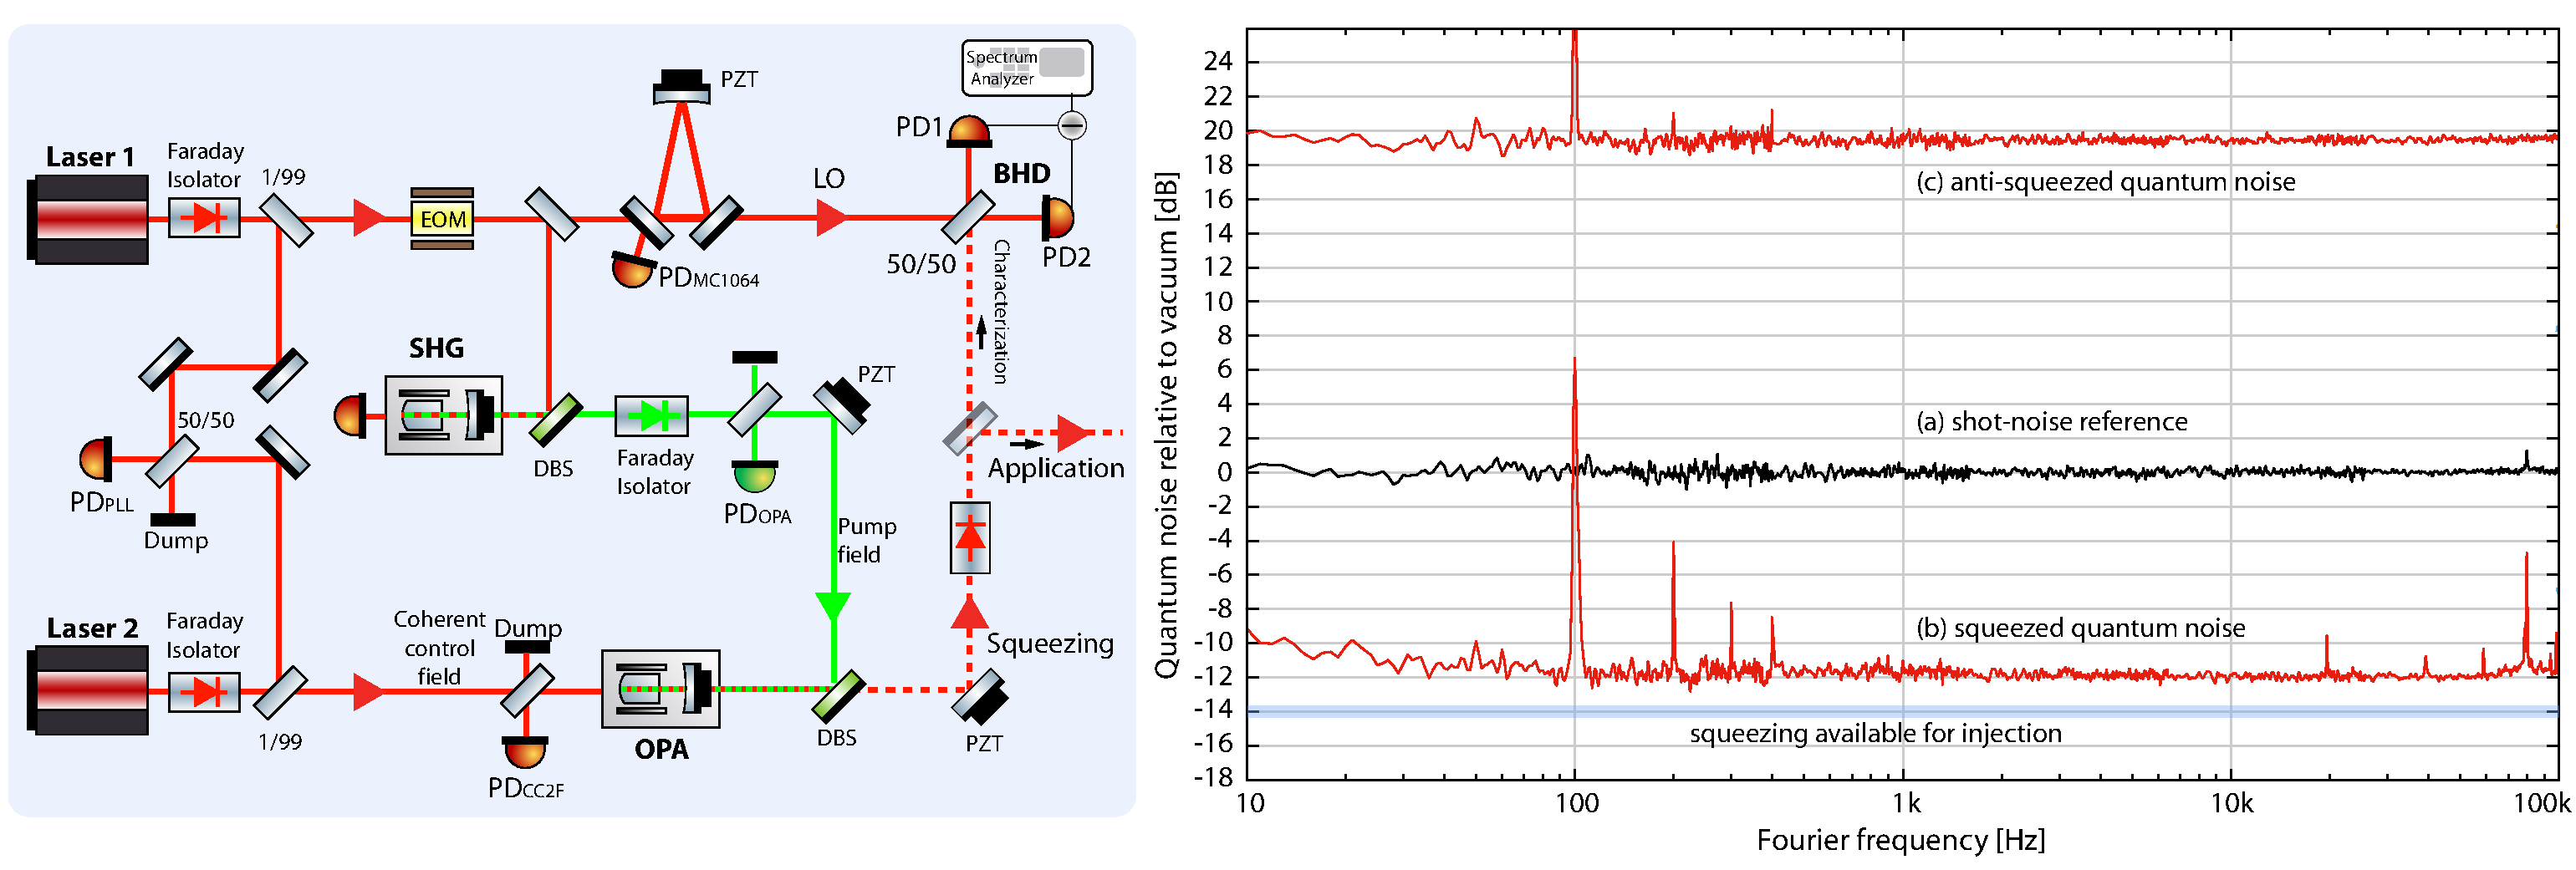
\includegraphics[width=\linewidth]{Detector/DetFigures/SqueezerFig1b.pdf}}
\caption{{\bf{Left:}} Schematic for the generation and coherent control of squeezed vacuum states of light. Laser 1 provides the light field for homodyne detection and for frequency doubling in a second harmonic generator (SHG). The SHG provides the pump field required for the generation of squeezed vacuum states in an optical parametric amplifier (OPA) operated below threshold. The squeezed vacuum states are extracted via a dichroic beam splitter (DBS) and send towards the interferometer. Alternatively, the squeezing level can be characterized by means of a balanced homodyne detector (BHD).  A Faraday isolator is implemented in the squeezing path to protect the OPA from light scattered back from the interferometer.\\
{\bf{Right}}: Quantum noise squeezing as reported in \cite{Mehmet2018}. Trace (a) represents the shot noise reference (normalized to 0\,dB) measured with a homodyne detector. In reference to this trace the measured quantum noise powers for squeezing (b) and the corresponding anti-squeezing (c) are shown.
Up to 12\,dB squeezing and 19.6\,dB anti-squeezing was observed, which is consistent with a theoretical model assuming a residual phase noise of 3.5\,mrad rms and an overall optical loss of 5.3\,\% for the squeezed field. This includes 2.5\,\%  optical loss due to the homodyne detection which needs to be subtracted to deduce the squeezing level available for the injection into a gravitational wave detector. This level is indicated by the blue area and corresponds to a squeezing factor of 14\,dB.}
\label{SqueezerFig1}
\end{figure}
%
The strongest squeezing level demonstrated to date is a squeeze factor of 15\,dB below the classical shot-noise limit at the wavelength of 1064\,nm, but only measured at MHz frequencies~\cite{Vahlbruch2016}. The topology of the optical parametric amplifier (OPA) used therein was a linear, standing-wave, doubly-resonant cavity with a non-linear crystal made from periodically poled potassium titanyl phosphate (PPKTP).  
%
Up to 13\,dB of non-classical noise suppression was measured at a wavelength of 1550\,nm~\cite{Schonbeck18} in a similar cavity design, but again only at MHz frequencies. 
%
By the implementation of a coherent control scheme \cite{Vahlbruch2006} and the mitigation of parasitic interferences the frequency band of detectable squeezing can be extended from MHz down to the required GW-frequencies \cite{Vahlbruch2007}. 
This has been demonstrated in tabletop experiments with various squeezed light source setups operated in-air or in-vacuum and with OPAs constructed as bow-tie or linear resonators \cite{Vahlbruch2006,Stefszky2012, Wade2016}.
%
Following these developments, similar schemes were used to realize squeezing enhancement in large scale gravitational wave detectors. 
The first successful implementation was achieved at the GEO600 detector in 2010 and since then squeezing has been routinely applied \cite{2011_Nat.Phys.7.962_LSC, Grote2013}. 
The Advanced Virgo and the two Advanced Ligo detectors have been also upgraded to include the squeezing technique since the O3 science run in early 2019.  
%

The highest squeezing level at GW-frequencies so far was reported in 2018 \cite{Mehmet2018}. Figure \ref{SqueezerFig1} summarizes the main result of this work, where squeezed light was generated in a linear, doubly-resonant OPA at a wavelength of 1064\,nm. A quantum noise reduction of up to 12\,dB at Fourier frequencies between 10\,Hz and 100\,kHz was directly measured with a diagnostic homodyne detector. The analysis revealed that the measured squeezing level corresponds to an equivalent squeezing factor of up to 14\,dB available for the injection into a gravitational wave detector with only 3.5\,mrad rms of phase noise attributed to the squeezed light source operated in air.The recent progress in the development of low-loss Faraday isolators \cite{Genin2018} suggests that this squeezing factor can be even further improved in the near future.
%
The available squeezing level and the intrinsic low phase noise are key parameters, since the obtainable effective squeezing level in the interferometer is limited by the overall amount of optical loss and phase noise as illustrated in Fig.\ref{QNSQZvsPNandloss}. 
%
With the demonstrated squeezing level and phase stability of the squeezed light source reported in \cite{Mehmet2018} it seems feasible to realize the envisaged squeezing enhancement of 10\,dB (effective) in ET-HF, which is listed as baseline parameter in Tab.\ref{tab:summary14}. 
 
For ET-LF, which will be operated at the wavelength of 1550\,nm, high squeezing levels at audio-band frequencies still need to be demonstrated. The realization of a suitable squeezed light source will rely on the same building blocks as developed and demonstrated for the ET-HF squeezer technology. First experiments reporting squeezing down to kHz-frequencies at 1550\,nm have already been conducted \cite{Mehmet2011,Schoenbeck2018phd}.

A total of six independent squeezed light sources will need to be engineered for ET: Three systems will generate squeezing at 1550\,nm for the ET-LF detector and three systems operating at 1064\,nm will be used for the ET-HF detectors. 


\bluecomment{SS: with the 532nm pump light, degradation of optics/crystals over time seems to be an issue. Has there been progress on this or are concepts foreseen that might reduce downtime? Do we expect better long-term performance at 775nm?}
\textcolor{red}{Important topic but maybe out-of-scope for this chapter. We prefer not to include this as there are so far no publications which can be used as references.}

\section {Newtonian Noise Cancellation}
% author Jan Harms
\label{Sec:NewtonianNoise}
\FloatBarrier
\label{sec:mitigateNN}
Local environmental mass-density fluctuations produce so-called Newtonian noise (NN) in a gravitational-wave detector through direct gravitational coupling with its test masses. Density perturbations can be associated with seismic, sound, temperature, and humidity fields, but also be produced by moving and vibrating objects. Newtonian-noise cancellation comprises techniques where auxiliary sensors are deployed to monitor sources of density perturbations, and their data are then used to produce a NN estimate that is being subtracted from the GW detector data.

As described in Section \ref{SiteReq}, the first step of any NN mitigation strategy is to reduce environmental disturbances. For ET, this includes site selection, underground construction, and realizing a low-noise detector infrastructure. However, only if the natural environment is among the quietest in the world, and excess anthropogenic noise can be avoided, then it might be possible to achieve the ET sensitivity target without NN cancellation. Nonetheless, without a detailed understanding of the seismic field, which is hard to obtain even with an extensive site-characterization study, NN modeling uncertainties are significant. It is therefore necessary to include NN cancellation in the R\&D plans.
\begin{figure}[t!]
    \centering
    \includegraphics[width=0.49\textwidth]{./Detector/NewtonianNoise/NewtonianNoiseFigures/Seismic_Surf.pdf}
    \includegraphics[width=0.49\textwidth]{./Detector/NewtonianNoise/NewtonianNoiseFigures/Seismic_UG.pdf}
    \caption{Estimates of seismic NN for ET. Left: ET constructed at the surface. Right: ET constructed underground. Plot from \cite{BaHa2019}.}
    \label{fig:NNestimates}
\end{figure}

As shown in Figure \ref{fig:NNestimates}, NN from surface waves will be strongly suppressed if the detector is constructed a few 100\,m underground. However, the NN from seismic body waves cannot be avoided at any depth, and it becomes a sensitivity-limiting noise contribution below 10\,Hz. Depending on the quality of the underground site, one still needs to mitigate body-wave NN by up to a factor 10. The range of body-wave NN shown in the two plots assumes that underground seismic spectra are a factor 3 to 12 above the global low-noise model \cite{Pet1993}, and an isotropic field is composed entirely of compressional waves. If it were composed entirely of shear waves, then the NN would be a factor 2 smaller. The prediction of Rayleigh NN (denoted {\it Surface} in the two plots) in underground detectors requires an assumption about the seismic surface spectrum, which is a factor 50 to 1000 above the global low-noise models in the two plots, but also an assumption about the dispersion curve. The slower (and therefore shorter) Rayleigh waves, the stronger is the suppression of associated NN with depth \cite{Har2015}. The dispersion model used for the two plots (Rayleigh wavelength plays a negligible role for NN in surface detectors) yields a Rayleigh-wave speed of 1.5\,km/s at 1\,Hz falling to 300\,m/s at 10\,Hz. There can be significant regional variations, but these values are typical. For the body-wave and Rayleigh-wave field, anisotropy can increase or decrease NN relative to the isotropic level shown in Figure \ref{fig:NNestimates}.

\subsection{Coherent noise cancellation}
\label{sub:Wiener}
The basic idea for noise cancellation is to exploit correlations between NN and data from a set of auxiliary sensors. An effective technique is to use Wiener filters \cite{Orf2007}. They are the optimal linear filters for this purpose provided that all time series are stationary, and they are effective even in the presence of non-stationary features in the data. Wiener filters can be estimates from data. It requires the calculation of correlations between all auxiliary sensors monitoring the environment, which form a correlation matrix $\mathbf C_{\rm SS}$, and between auxiliary sensors and GW detector, which form a vector $\vec C_{\rm SN}$. Since one is mostly interested in the frequency-domain representation of detector noise, correlations are expressed as cross-spectral densities depending on frequency $\omega$. The Wiener filter can then be written
\begin{eqnarray}
		\vec w(\omega)=\mathbf C_{SS}(\omega)^{-1}\cdot\vec C_{\rm SN}(\omega)
		\label{eq:Wiener}
\end{eqnarray}
This filter is applied to discrete Fourier transforms of data from auxiliary sensors, $\vec d(\omega_i)$, to produce an estimate $\hat n(\omega_i)=\vec w(\omega_i)^\dagger\cdot \vec d(\omega_i)$ of NN, which is then subtracted from the GW detector data. In average, the relative suppression of NN by a Wiener filter is given by
\begin{eqnarray}
		\epsilon(\omega)=\sqrt{1-\frac{\vec C^\dagger_{\rm SN}(\omega)\cdot \mathbf C_{\rm SS}(\omega)^{-1}\cdot\vec C_{\rm SN}(\omega)}{C_{\rm NN}(\omega)}},
		\label{eq:residual}
\end{eqnarray}
where $C_{\rm NN}(\omega)$ is the spectral density of NN in the GW detector. This expression tells us that to achieve a good subtraction efficiency, three conditions are to be met:
\begin{itemize}
\item All the sensors should be coupled as much as possible to NN. In other words, the correlation $\vec C_{\rm SN}$ between sensor outputs and GW detector must be large.
\item The correlations between sensors, described by the matrix $\mathbf C_{\rm SS}$, which also include sensor noise on its diagonal, must be small.
\end{itemize}
Designing a NN cancellation system for a GW detector that is yet to be built, only the correlations among auxiliary sensors $\mathbf C_{\rm SS}$ can be measured during a site-characterization campaign. A model is required using the correlations $\mathbf C_{\rm SS}$ to obtain $\vec C_{\rm SN}$ and $C_{\rm NN}$ \cite{CoEA2016a}.

The theory of Wiener filtering does not directly address a major challenge of NN cancellation, which is the optimal placement of auxiliary sensors. This aspect is very important for the cancellation of NN from seismic and atmospheric fields. Analyses of optimal array configurations are important since, even when lacking an accurate understanding of environmental fields, optimization results provide useful estimates of the required number of auxiliary sensors, the required sensitivity of sensors, and an approximate idea of how far from the test masses sensors need to be placed. This aspect is discussed in Section \ref{sub:optimization}.

\subsection{Site properties relevant to Newtonian-noise cancellation}
\label{sub:properties}
Since the Wiener filter is based on correlations in environmental fields, anything that influences these correlations affects NN cancellation. In the following, site properties relevant to seismic and atmospheric NN are briefly described.

\subsubsection*{Seismic fields}
\begin{itemize}
\item {\bf Seismic speed}\; Seismic correlations and correlations of seismic NN between test masses decrease with increasing distance. In frequency domain, this can be quantified in terms of a spatial correlation function $\mathcal F$ that assumes its maximal value 1 when the two seismometers or test masses are sharing the same location. As a function of the separation $L$, one finds for isotropic Rayleigh-wave fields
\begin{eqnarray}
	\mathcal{F}_{\rm NN}=J_{0}(2\pi L/\lambda)-J_{2}(2\pi L/\lambda),\quad \mathcal{F}_{\rm seis}=J_{0}(2\pi L/\lambda).
	\label{eq:geometrical}
\end{eqnarray}
As is intuitively clear, how quickly correlation decreases with increasing distance $L$ depends on the length $\lambda$ of a Rayleigh wave. The first zero of the seismic correlation is at a distance of about $0.4\lambda$. Correlations of NN between two test masses of one arm separated by several kilometers can be neglected. Due to equation (\ref{eq:residual}), seismometer arrays used for NN cancellation ideally have diameters similar to the length a Rayleigh wave. 

\item {\bf Wave polarizations}\; Seismic-wave polarizations play a major role in NN cancellation. The two main polarizations are shear and compressional waves, and Rayleigh surface waves are a so-called inhomogeneous (amplitude decreasing exponentially with depth) extension of a superposition between these two polarizations. The composition of the seismic field in terms of wave polarizations varies between sites, and depends on local geology as well as on the type and location of seismic sources. All polarizations produce NN either through compression of the medium or by displacement of surfaces and interfaces.

If only one wave polarization is present at a time, then it is almost trivial to cancel associated NN \cite{Har2015,HaVe2016}. A mix of wave polarizations can however make it very difficult to cancel a significant amount of NN \cite{HaVe2016,BaHa2019}. The issue is that correlations between seismometers and test mass decrease more quickly with distance when multiple polarizations are present, which hampers efficient noise cancellation as pointed out in Section \ref{sub:Wiener}. As a consequence, a larger number of seismometers is required to be able to be distinguish between polarizations and be susceptible to the correlations of each wave type. 

\item {\bf Seismic sources}\; The distribution and type of seismic sources both influence the composition of a seismic field. Most important to know is whether seismic sources are local or distant, and whether they are underground or at the surface. Some sources might not even fall into a clear category if it is for example a surface structure anchored to a deeper part of the ground. With respect to environmental noise, it is one of the most important tasks of a site-characterization campaign to identify as many seismic sources as possible. A NN cancellation scheme can be greatly simplified or be made significantly more effective if understanding about the seismic sources is used. Furthermore, excess noise produced by the infrastructure of the Einstein Telescope will also pose additional challenges for the design of a NN cancellation system. 

\item {\bf Local topography and geology}\; Two-point correlations of the seismic field can be affected by topography and geology. Generally, seismic-wave reflections from surfaces and interfaces cause conversions between wave polarizations. Scattering from non-planar structures can also give rise to local field components that strongly decay with distance. These local components are very similar in nature to the near-field of seismic sources. In the presence of significant geological heterogeneities or rough surface topography, it is therefore more challenging to collect all information required to design seismometer arrays for efficient NN cancellation \cite{CoHa2012}. Especially in relatively noisy environments with elevated NN where more efficient cancellation of NN might be required, site characterization should therefore assess geological properties and topography also in the context of NN cancellation.

\end{itemize}

\subsubsection*{Atmospheric fields}
Avoiding NN from the atmosphere is an important reason to construct the Einstein Telescope underground. In Section \ref{sec:envnoise}, some of the complexity of atmospheric fields and how they produce NN are described. There are serious practical challenges to design a cancellation system for atmospheric NN. 

\begin{itemize}
\item {\bf Wind noise}\; The variety of phenomena makes the monitoring of the atmosphere a challenging task. One strategy for NN cancellation would be to monitor sound, wind speed, temperature and humidity fields. Sound is typically measured with microphones. However, pressure fluctuations produced by turbulent flow in the vicinity of a microphone can mask an underlying sound signal \cite{Gre2015}. This contribution is often called wind noise. Clever sensor design, averaging pressure signals over some baseline, or constructing wind shields can prove effective \cite{Ell1972,WaHe2009,NoEA2014}. However, when it comes to an order of magnitude suppression of NN from sound, then even a small incoherent contribution to signals from wind noise can be detrimental. For this reason, entirely new approaches need to be considered. 

\item {\bf LIDAR}\; LIDAR (derived from \emph{light} and \emph{radar}) technology has been applied to investigate microscale physics in the atmospheric boundary layer. It consists of a laser beam that scatters back from the atmosphere carrying information about the presence of certain molecules, or wind speed \cite{CLN2004}, temperature \cite{Beh2005}, etc. Volumetric observations can be performed to characterize the evolution of entire fields. It is conceivable that a LIDAR system can be developed in the foreseeable future to cancel at least modest amounts of wind-driven NN associated with temperature and humidity fields. However, atmospheric density perturbations due to sound are orders of magnitude weaker in the ET observation band, which makes it extremely challenging to develop a LIDAR to monitor sound fields.

\item {\bf Cavity atmosphere}\; Potentially significant NN contributions can come from the sound field inside the cavities hosting the test masses of the Einstein Telescope \cite{FiEA2018}. Due to the absence of fast air currents, wind noise in microphones located inside the cavity will be strongly reduced, and high-precision sound monitoring would be possible. At the same time, absence of fast air currents also means that all forms of cavity atmospheric NN driven by wind, i.e., associated with temperature and humidity fields, will be negligible. This means that cancellation from cavity atmospheric NN should be possible using an array of microphones.
\end{itemize}

\subsection{Optimized sensor arrays for seismic NN cancellation}
\label{sub:optimization}

Another important point to understand is how the subtraction procedure improves with the number of sensors, and how much it is sensitive to a non optimal placement of the sensors. This is important because in a practical implementation, the possibility of optimizing the placement of underground sensors will be limited. 

Optimized seismometer arrays were initially studied for the cancellation of NN from Rayleigh waves \cite{DHA2012,Har2015,CoEA2016a}, and more recently from body waves \cite{BaHa2019}. Array optimization was based on simplified models of the seismic field in all these publications, which means that the calculated array configurations are not of direct use for NN cancellation in real environments. However, the total number of seismometers and the seismometer sensitivity required to achieve a certain cancellation performance are less dependent on the model of the seismic field \cite{CoEA2016a}. 

Accordingly, Fig.~\ref{fig:residualN} gives an estimate of the required number of seismometers to cancel a certain amount of body-wave NN provided that they assume their optimal positions. 
\begin{figure}[t!]
	\begin{center} 
		\includegraphics[width=0.7\textwidth]{./Detector/NewtonianNoise/NewtonianNoiseFigures/SNR_ch3.png} 
		\caption{Suppression of body-wave NN as a function of number of seismometers with optimal placement. The seismometers measure seismic signals with an SNR of 15. The black curve shows the lowest possible residual determined by the seismometer SNR without considering properties of the seismic field. Plot from \cite{BaHa2019}.} 
		 \label{fig:residualN} 
	\end{center}
\end{figure}
About 15 seismometers are required to achieve a factor 10 suppression. It should be emphasized that this result depends to some extent on the relative contributions of compressional waves and shear waves to the seismic field. For these results, it is assumed that compressional waves constitute 30\% of the seismic power-spectral density. Less seismometers are required if one polarization greatly dominates over the other. These instruments need to be deployed in boreholes, and the number 15 is per test mass. 

In this context, one can now address the question how accurately the seismometers need to be placed with respect to their optimal locations. While direction and vertical drilling technology has become increasingly accurate \cite{MCZ2016}, significant deviations from optimal drilling are to be expected, which results in sub-optimal seismometer placements. Figure \ref{fig:errorNN} shows the residuals that can be achieved with sub-optimal seismometer placement. 
\begin{figure}[t!]
	\begin{center} 
		\includegraphics[width=0.7\textwidth]{./Detector/NewtonianNoise/NewtonianNoiseFigures/errorbody.png} 
		\caption{Suppression of NN from body waves with 15 single-axis (ch1) and three-axis (ch3) seismometers. Sensor locations of 500 arrays for each histogram are derived from the optimal array by adding random numbers to all optimal coordinates drawn from Gaussian distributions of width $\sigma$. Vertical lines mark the residual of the optimal arrays. Plot from \cite{BaHa2019}.} 
		 \label{fig:errorNN} 
	\end{center}
\end{figure}
To produce this plot, seismometer coordinates were shifted by a random number drawn from a Gaussian distribution of width $\sigma$ specified in the legend relative to the length $\lambda$ of compression waves. Assuming a compressional-wave speed of 4\,km/s, $\sigma=0.07\lambda=28\,$m at 10\,Hz. The corresponding arrays with three-axis sensors (ch3) still achieve a body-wave NN suppression by a factor 3 and better. For boreholes of a few 100\,m, and drill deviation of less than 1 degree, such sensor-placement accuracy is achievable. 

The remaining challenge is to have sufficient observations of the seismic field to be able to accurately calculate the optimal array configurations. In fact, incomplete knowledge of seismic correlations will likely lead to the dominant error in the seismometer placements. This error needs to be minimized by studying in detail the seismic field at the site of the Einstein Telescope also using borehole seismometer installations.
